\subsection{Stored Functions}

This section presents two stored functions used to calculate business values from the database. 
Unlike stored procedures, these functions return a single calculated value and can be used directly inside \texttt{SELECT} statements.

The first function calculates the total spending of a player within a selected date range. 
The second function calculates the net revenue of a developer after subtracting the platform fee. 
Both functions include input validation and use cursors to process related records step by step.
\subsubsection{Function 1: Calculate Player Spending}

The function \texttt{fn\_CalculatePlayerSpending} calculates the total amount spent by a player within a selected date range. 
It receives a player ID, a starting date, and an ending date as input parameters.

The function first validates the input values. 
It checks whether the player ID is empty, whether the player exists, whether the date range is empty, and whether the starting date is later than the ending date. 
After validation, it uses a cursor to iterate through all transactions of the selected player within the given period and accumulates the transaction amounts into a total spending value.

This function is useful for player-side analysis, such as showing how much a player has spent on the platform during a specific period.
\subsubsection{Function 2: Calculate Developer Net Revenue}

The function \texttt{fn\_GetDeveloperNetRevenue} calculates the net revenue of a developer within a selected date range after subtracting a platform fee percentage. 
It receives a developer ID, a starting date, an ending date, and a platform fee percentage as input parameters.

This function is more advanced because it uses a cursor to iterate through all games published by the selected developer. 
For each game, it calculates revenue from base game sales using the \texttt{CONTAINS} table and revenue from DLC sales using the \texttt{BUY\_DLC} and \texttt{DLC} tables. 
The game revenue and DLC revenue are accumulated into gross revenue. 
Finally, the platform fee is subtracted to return the developer's net revenue.

The function also validates important input conditions, including developer existence, valid date range, and valid platform fee percentage.
\subsubsection{Full SQL Implementation}

The following SQL script shows the full implementation of the two stored functions.

\begin{lstlisting}[language=SQL, caption={Stored functions for player spending and developer net revenue}, label={lst:stored-functions}]
USE steam_store;

DELIMITER //

DROP FUNCTION IF EXISTS fn_CalculatePlayerSpending //

CREATE FUNCTION fn_CalculatePlayerSpending(
    p_player_id INT,
    p_from_date DATE,
    p_to_date DATE
)
RETURNS DECIMAL(14,2)
DETERMINISTIC
READS SQL DATA
BEGIN
    DECLARE done INT DEFAULT 0;
    DECLARE v_amount DECIMAL(14,2) DEFAULT 0;
    DECLARE v_total_spending DECIMAL(14,2) DEFAULT 0;

    DECLARE cur_player_transactions CURSOR FOR
        SELECT IFNULL(t.total_amount, 0)
        FROM `TRANSACTION` t
        WHERE t.player_id = p_player_id
          AND DATE(t.`date`) BETWEEN p_from_date AND p_to_date
        ORDER BY t.`date`;

    DECLARE CONTINUE HANDLER FOR NOT FOUND SET done = 1;

    IF p_player_id IS NULL THEN
        SIGNAL SQLSTATE '45000'
            SET MESSAGE_TEXT = 'Player ID cannot be empty.';
    END IF;

    IF NOT EXISTS (SELECT 1 FROM `PLAYER` WHERE user_id = p_player_id) THEN
        SIGNAL SQLSTATE '45000'
            SET MESSAGE_TEXT = 'Player ID does not exist.';
    END IF;

    IF p_from_date IS NULL OR p_to_date IS NULL THEN
        SIGNAL SQLSTATE '45000'
            SET MESSAGE_TEXT = 'Date range cannot be empty.';
    END IF;

    IF p_from_date > p_to_date THEN
        SIGNAL SQLSTATE '45000'
            SET MESSAGE_TEXT = 'From date cannot be later than to date.';
    END IF;

    OPEN cur_player_transactions;

    spending_loop: LOOP
        FETCH cur_player_transactions INTO v_amount;

        IF done = 1 THEN
            LEAVE spending_loop;
        END IF;

        SET v_total_spending = v_total_spending + v_amount;
    END LOOP;

    CLOSE cur_player_transactions;

    RETURN v_total_spending;
END //

DROP FUNCTION IF EXISTS fn_GetDeveloperNetRevenue //

CREATE FUNCTION fn_GetDeveloperNetRevenue(
    p_developer_id INT,
    p_from_date DATE,
    p_to_date DATE,
    p_platform_fee_percent DECIMAL(5,2)
)
RETURNS DECIMAL(14,2)
DETERMINISTIC
READS SQL DATA
BEGIN
    DECLARE done INT DEFAULT 0;
    DECLARE v_game_id INT;
    DECLARE v_game_sales DECIMAL(14,2) DEFAULT 0;
    DECLARE v_dlc_sales DECIMAL(14,2) DEFAULT 0;
    DECLARE v_gross_revenue DECIMAL(14,2) DEFAULT 0;
    DECLARE v_net_revenue DECIMAL(14,2) DEFAULT 0;

    DECLARE cur_developer_games CURSOR FOR
        SELECT g.game_id
        FROM `GAME` g
        WHERE g.developer_id = p_developer_id
        ORDER BY g.game_id;

    DECLARE CONTINUE HANDLER FOR NOT FOUND SET done = 1;

    IF p_developer_id IS NULL THEN
        SIGNAL SQLSTATE '45000'
            SET MESSAGE_TEXT = 'Developer ID cannot be empty.';
    END IF;

    IF NOT EXISTS (SELECT 1 FROM `DEVELOPER` WHERE user_id = p_developer_id) THEN
        SIGNAL SQLSTATE '45000'
            SET MESSAGE_TEXT = 'Developer ID does not exist.';
    END IF;

    IF p_from_date IS NULL OR p_to_date IS NULL THEN
        SIGNAL SQLSTATE '45000'
            SET MESSAGE_TEXT = 'Date range cannot be empty.';
    END IF;

    IF p_from_date > p_to_date THEN
        SIGNAL SQLSTATE '45000'
            SET MESSAGE_TEXT = 'From date cannot be later than to date.';
    END IF;

    IF p_platform_fee_percent IS NULL THEN
        SIGNAL SQLSTATE '45000'
            SET MESSAGE_TEXT = 'Platform fee cannot be empty.';
    END IF;

    IF p_platform_fee_percent < 0 OR p_platform_fee_percent > 100 THEN
        SIGNAL SQLSTATE '45000'
            SET MESSAGE_TEXT = 'Platform fee must be between 0 and 100.';
    END IF;

    OPEN cur_developer_games;

    revenue_loop: LOOP
        FETCH cur_developer_games INTO v_game_id;

        IF done = 1 THEN
            LEAVE revenue_loop;
        END IF;

        SELECT IFNULL(SUM(c.price_at_purchase), 0)
        INTO v_game_sales
        FROM `CONTAINS` c
        JOIN `TRANSACTION` t 
            ON c.transaction_id = t.transaction_id
        WHERE c.game_id = v_game_id
          AND DATE(t.`date`) BETWEEN p_from_date AND p_to_date;

        SELECT IFNULL(SUM(d.price), 0)
        INTO v_dlc_sales
        FROM `BUY_DLC` bd
        JOIN `DLC` d
            ON bd.game_id = d.game_id
           AND bd.dlc_name = d.dlc_name
        JOIN `TRANSACTION` t 
            ON bd.transaction_id = t.transaction_id
        WHERE bd.game_id = v_game_id
          AND DATE(t.`date`) BETWEEN p_from_date AND p_to_date;

        SET v_gross_revenue = v_gross_revenue + v_game_sales + v_dlc_sales;
    END LOOP;

    CLOSE cur_developer_games;

    SET v_net_revenue = v_gross_revenue * (1 - p_platform_fee_percent / 100);

    RETURN v_net_revenue;
END //

DELIMITER ;
\end{lstlisting}
\subsubsection{Test Cases}

The following SQL statements were used to test the stored functions. 
The first two test cases calculate total spending for two players. 
The last two test cases calculate net revenue for two developers after applying a 30\% platform fee.

\begin{lstlisting}[language=SQL, caption={Test cases for stored functions}, label={lst:function-test-cases}]
SELECT fn_CalculatePlayerSpending(
    1, 
    '2023-01-01', 
    '2024-12-31'
) AS player_1_total_spending;
SELECT fn_GetDeveloperNetRevenue(
    16, 
    '2023-01-01', 
    '2024-12-31', 
    30
) AS developer_16_net_revenue;
\end{lstlisting}
\subsubsection{Execution Result}
The execution results show that the functions return correct calculated values based on the sample data. 
The player spending function returns the total amount spent by each selected player during the given period. 
The developer net revenue function returns the revenue after subtracting the platform fee from gross game and DLC sales.

\begin{figure}[H]
    \centering
    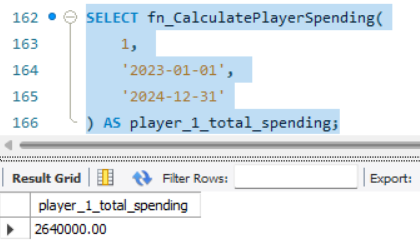
\includegraphics[width=0.6\linewidth]{graphics/function_player_spending_result.png}
    \caption{Result of calculating total player spending using stored functions}
    \label{fig:function-player-spending-result}
\end{figure}

\begin{figure}[H]
    \centering
    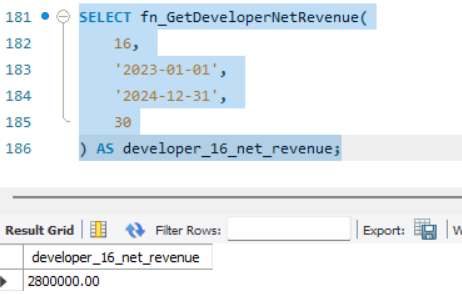
\includegraphics[width=0.6\linewidth]{graphics/function_developer_revenue_result.png}
    \caption{Result of calculating developer net revenue using stored functions}
    \label{fig:function-developer-revenue-result}
\end{figure}